\section{Examples of the Preceding Method}

We will use these nativities as examples in order to make our system understandable to our readers: \Sun, \Moon, \Venus, \Mercury, Ascendant in \Scorpio, \Saturn\xspace in \Sagittarius, \Jupiter\xspace in \Capricorn, \Mars\xspace in \Leo\footnote{\textit{Greek Horoscopes} dates the chart to November 14, 134CE, sunrise}. 

\begin{wrapfigure}[14]{R}{7cm}
\centering
\vspace{-20pt}
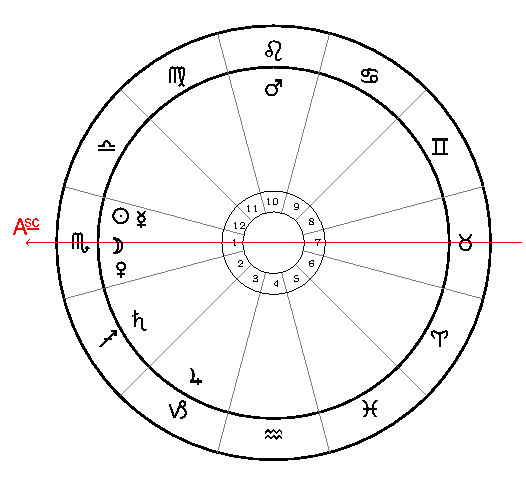
\includegraphics[width=.68\textwidth]{charts/5_10_01}
\caption{Chart 56 [V.10.1, GH L134,XI]}
\label{fig:chart56}
\end{wrapfigure}

In the 20th year the transmission was from \Jupiter\xspace in \Capricorn\xspace to \Mars\xspace in \Leo, which are 8 signs
apart. \Jupiter\xspace in the third sign <from the Ascendant> transmitted to \Mars\xspace \textbf{/228K/} in the tenth sign, MC.
A petition for higher rank was submitted to the king but did not succeed, because the transmission from \Jupiter\xspace to \Mars\xspace is grievous. 

The distribution by 4 signs is also strong, from \Mars\xspace to the \Sun, \Moon, Ascendant, \Mercury, and \Venus. He was ill in his 20th year: after falling from an animal he was dragged so badly as to almost lose his eyesight. With regard to a female he suffered gossip, assaults, and a penalty, so that each star had its own effect when it received the chronocratorship from the malefic. 

In his 23rd year \Jupiter\, transmitted from the Kingly Place (the III and the IX Places from the Ascendant indicate God and king) to the luminaries, \Venus, the Ascendant, and \Mercury\footnote{These are eleven (23 - 12 = 11) signs from \Jupiter.}, and they provided him with a powerful ally by means of gifts\footnote{Schmidt notes that this probably means the native was given a place on a council in exchange for gifts.}. Nothing can give a man friendship with kings and the great if the chronocrators are against it.

Another example: \Sun\xspace in \Taurus, \Moon, \Mercury\xspace in \Aries, \Saturn\xspace in \Pisces, \Jupiter, \textbf{/217P/} \Mars\xspace in \Aquarius, \Venus\xspace in \Gemini, Ascendant in \Virgo\footnote{\textit{Greek Horoscopes} dates the chart to April 24, 111CE at about 2pm. And computes \Jupiter\xspace at 27 \Capricorn}. 

\begin{wrapfigure}[15]{R}{7cm}
\centering
\vspace{-20pt}
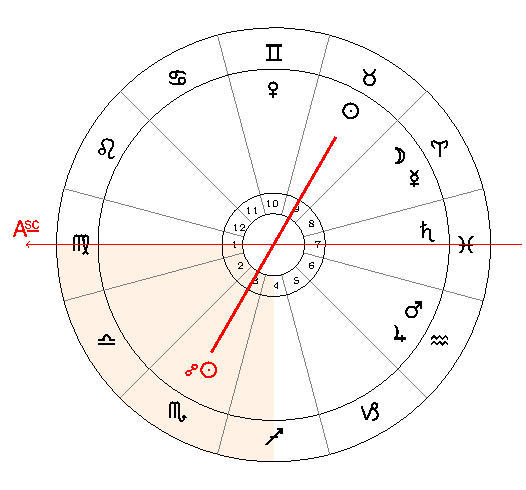
\includegraphics[width=.68\textwidth]{charts/5_10_02}
\caption{Chart 57 [V.10.2, GH L111,IV]}
\label{fig:chart57}
\end{wrapfigure}

In his 42nd year he was the heir of a female because the transmission by 6 signs \textsl{[42 - (3 x 12)]} was from the \Moon\xspace and \Mercury\xspace in the <VIII> Place of Death, \Aries, to \Virgo\xspace <the Ascendant>, the house of \Mercury, and from a sign of exaltation <of the \Sun, \Aries> to an exaltation <of \Mercury, \Virgo>\footnote{The exaltation signs are likely of note because \Mercury\, is being disposted by the \Sun, the exaltation ruler of \Aries, and is himself the exaltation ruler of the sign (\Virgo) to which the transmission is being made.}. 

In his 45th year he had a distinguished office of public affairs, because \Venus\xspace at MC transmitted to \Mars, which indicates trouble, and to \Jupiter, which indicates high rank \footnote{There are 9 signs between the MC and \Jupiter\, and \Mars: 45 - (3 x 12) = 9}. The vital sector was also from the Ascendant to the \Sun\footnote{The Ascendant met with opposition of the \Sun\, which was within the vital sector? GH puts the \Sun\, at 2 \Taurus. Using ascension times of 40 for \Libra\, and 36 for \Scorpio, $\approx$ age would be 42y 5m plus some portion of \Virgo\, equivalent to 45 - 42.4 = 3.46, so Ascendant would need to have been around 26-27 \Virgo.}, and so he was recognized by the king at that time. In the same year he freed his concubines because \Jupiter, in the VI Place concerned with slaves, received the chronocratorship from \Venus. 

In his 46th year \textsl{[46 - (3 x 12) = 10]} he had troubles and the disruption of <religious> matters, troubles because of females, and the deaths of two concubines, because the transmission was from \Venus\xspace to \Saturn\xspace in the Marriage-bringer <VII Place>, and from the \Sun\xspace to \Mars\xspace and \Jupiter. He escaped from these disturbances.

\newpage
Another example: \Sun\xspace in \Taurus, \Moon, \Venus, Ascendant in \Aries, \Saturn\xspace in \Capricorn, \Jupiter\xspace in \Virgo, \Mars\xspace in \Scorpio, \Mercury\xspace in \Gemini\footnote{\textit{Greek Horoscopes} gives the date as May 8, 107CE about 4 a.m.}. 

\begin{wrapfigure}[15]{R}{7cm}
\centering
\vspace{-20pt}
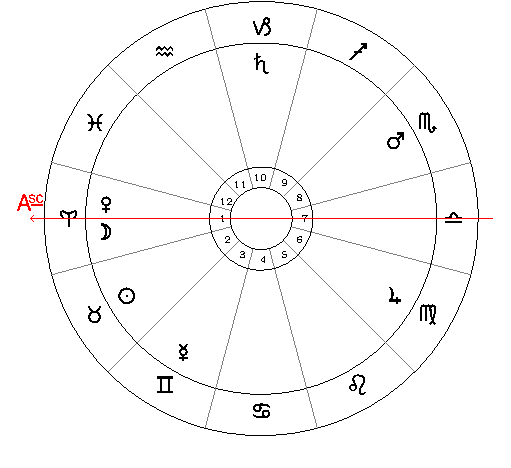
\includegraphics[width=.68\textwidth]{charts/5_10_03}
\caption{Chart 58 [V.10.3, GH L107]}
\label{fig:chart58}
\end{wrapfigure}


In his 51st year he travelled abroad, and going before the king he won a lawsuit \textbf{/229K/} for a high-priesthood on behalf of a friend. The transmission from the \Moon, \Venus, and the Ascendant was to \Mercury\xspace in <the III Place of> the Goddess and king. In the same year the death of a child occurred, because \Mars\xspace in the <VIII> Place of Death transmitted to \Saturn\xspace in the <X> Place associated with children.

\begin{wrapfigure}[11]{R}{7cm}
\centering
\vspace{-40pt}
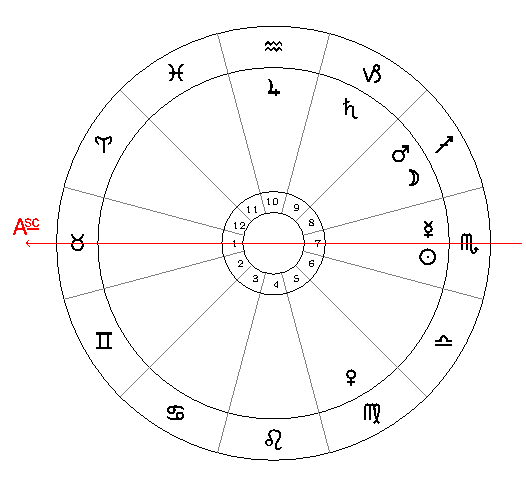
\includegraphics[width=.68\textwidth]{charts/5_10_04}
\caption{Chart 59 [V.10.4, GH L135,X]}
\label{fig:chart59}
\end{wrapfigure}

\noindent Another example: \Sun, \Mercury\xspace in \Scorpio, \Moon, \Mars\xspace in \Sagittarius, \Saturn\xspace in \Capricorn, \Jupiter\xspace in \Aquarius, \Venus\xspace in \Virgo, Ascendant in \Taurus\footnote{\textit{Greek Horoscopes} gives the date as October 27, 135CE about sunset.}. 

The horoscope of the son of the father (whose horoscope immediately preceded) is given for comparison. Using this distribution he comes to his 22nd year in agreement with his father’s horoscope. \Jupiter\xspace made the transmission to the \Sun, i.e. to the father, and the transmission from \Mars\xspace in the <VIII> Place of Death to \Venus\xspace was the cause of death.

Another example: \Sun, \Mars, \Venus\xspace in \Leo, \Moon\xspace in \Aquarius, \Saturn\xspace in \Aries, \Jupiter\xspace in \Pisces,
\Mercury\xspace in \Cancer, Ascendant in \Virgo\footnote{\textit{Greek Horoscopes} gives the chart date as July 27, 112 at about 8 a.m.}. 

\begin{wrapfigure}[15]{R}{7cm}
\centering
\vspace{-20pt}
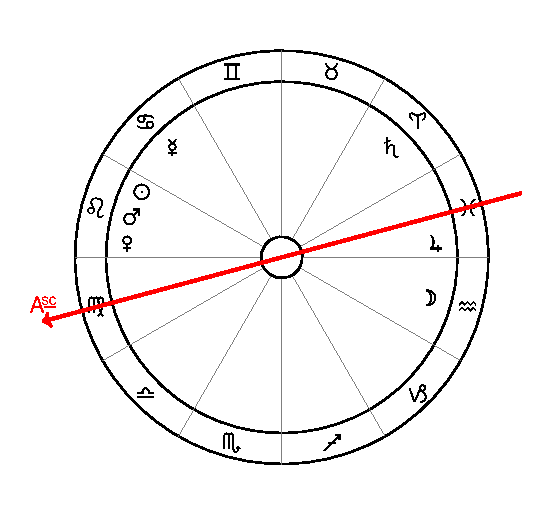
\includegraphics[width=.68\textwidth]{charts/5_10_05}
\caption{Chart 60 [V.10.5, GH L112,VII]}
\label{fig:chart60}
\end{wrapfigure}


In his 24th year he profited from legacies and friends. In his 26th
year, marriage and help from a women. In his 29th year he had trouble and disturbances because of the death of someone else’s slave and a charge of poisoning, because \Saturn\xspace made the transmission to the \Sun, \Mars, and \Venus\xspace in the <XII> Place associated with slaves. 

He found \textbf{/218P/} help through his friendship with the great, both males and females. In his 31st year he travelled, and while abroad he managed pleasantly and profitably at the start, but later he seduced a slave and experienced jealousy and quarrels, because the transmission was from the \Sun, \Venus, and \Mars (in the <XII> Place associated with slaves) to the \Moon, and from the Ascendant to \Jupiter\xspace in the Marriage-bringer <VII Place>. 

In his 33rd year he was ejected from a ship <?> and condemned to be a slave. Even though convicted, he found kindness because
of the transmission from \Mercury\xspace to \Jupiter. The term of imprisonment, however, is made obvious because of the sextile aspect of the \Moon\xspace with \Saturn\xspace (as we have previously explained), and because the chronocratorship passed from \Mars\xspace and the \Sun to the Crisis-producing Place <VIII Place>, i.e. to \Saturn, causing the conviction. 

In his 45th year he was released through the influence of great individuals on the grounds of illness; the transmission <by 9 signs> of the previous chronocrator <at age 33> and of this one <age 45> was a mixture of benefic and malefic. But the malefics were retrograde <\Saturn>, under the rays of the \Sun\xspace <\Mars>, and becoming dim, and they fell in rather weak Places.
Consequently it will be necessary to examine the transmission of all the stars /230K/ to see if the transmissions of malefics or of benefics predominate, or if they are mixed. Having done this, make the forecast. 

\begin{wrapfigure}[15]{R}{7cm}
\centering
\vspace{-20pt}
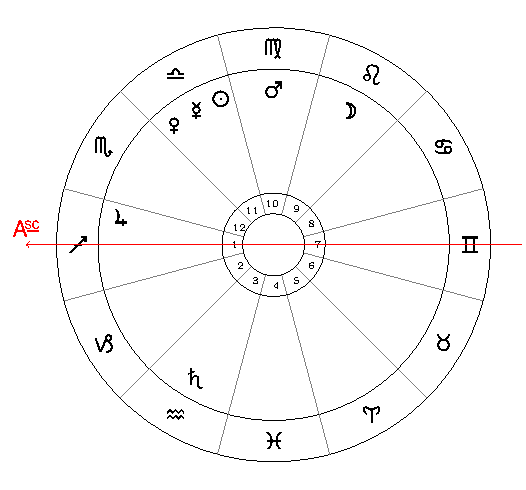
\includegraphics[width=.68\textwidth]{charts/5_10_06}
\caption{Chart 61 [V.10.6, GH L110,IX]}
\label{fig:chart61}
\end{wrapfigure}

\noindent We have explained this in our instructions; so as not to seem verbose, we have appended the following condensed horoscopes. The reader can interpret the places and the causative forces by using the
explanations which have been or will be given: \Sun, \Mercury, \Venus \xspace in \Libra, \Saturn\xspace in \Aquarius, \Jupiter, Ascendant in \Sagittarius, \Mars\xspace in \Virgo, \Moon in \Leo\footnote{\textit{Greek Horoscopes} dates the chart to September 27, 110 CE at about 10 a.m.}. 

In his 47th year he was the heir of a friend, and in the same year he was separated from his wife because of jealousy and abuse.

\begin{wrapfigure}[10]{R}{7cm}
\centering
\vspace{-20pt}
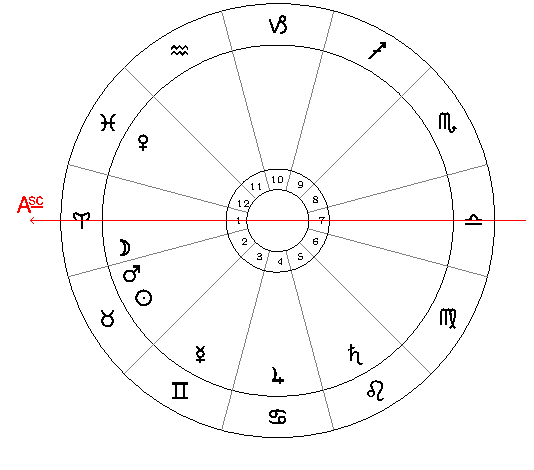
\includegraphics[width=.68\textwidth]{charts/5_10_07}
\caption{Chart 62 [V.10.7, GH L153]}
\label{fig:chart62}
\end{wrapfigure}

\noindent Another example: \Sun, \Mars\xspace in \Taurus, \Moon, Ascendant in \Aries, \Saturn\xspace in \Leo, \Jupiter\xspace in \Cancer, \Venus\xspace in \Pisces, \Mercury\xspace in \Gemini\footnote{\textit{Greek Horoscopes} dates the chart to May 8, 153 CE at about 4 a.m.}. 

In his fourth year the death of his father occurred.

\vspace{1.2cm}

\begin{wrapfigure}[13]{R}{7cm}
\centering
\vspace{-20pt}
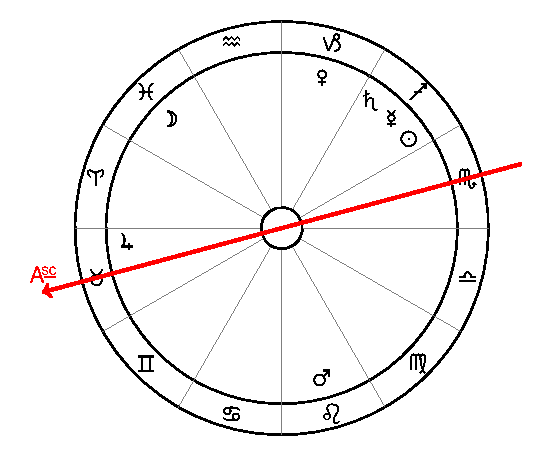
\includegraphics[width=.68\textwidth]{charts/5_10_08}
\caption{Chart 63 [V.10.8, GH L102,XII,4]}
\label{fig:chart63}
\end{wrapfigure}

\noindent Another example: \Sun, \Mercury, \Saturn\xspace in \Sagittarius, \Moon in \Pisces, \Mars\xspace in \Leo, \Venus\xspace in \Capricorn, Ascendant, \Jupiter\xspace in \Taurus. 

In his 45th year twin children were still-born <?>. In the same
year he became a high-priest. In his 51st year a distinguished public office. In his 52nd year the death of a child. 

\begin{wrapfigure}[14]{R}{7cm}
\centering
\vspace{-20pt}
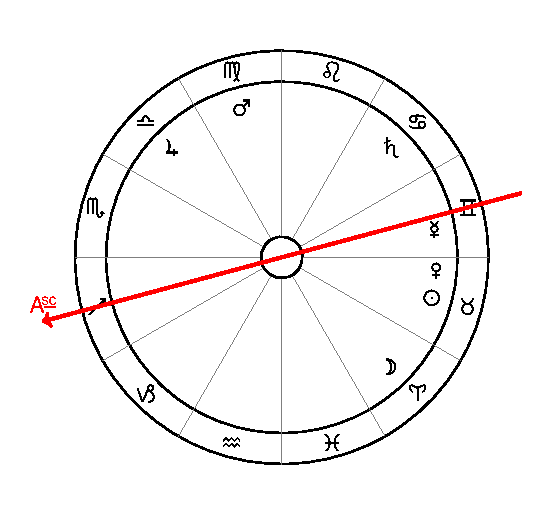
\includegraphics[width=.68\textwidth]{charts/5_10_09}
\caption{Chart 64 [V.10.9, GH L120,V]}
\label{fig:chart64}
\end{wrapfigure}

\noindent Another example: \Sun, \Venus\xspace in \Taurus, \Moon\xspace in \Aries, \Saturn\xspace in \Cancer, \textbf{/219P/} \Jupiter <in \Libra>, \Mars\xspace in \Virgo, \Mercury\xspace in \Gemini, Ascendant in \Sagittarius\footnote{\textit{Greek Horoscopes} dates the chart to May 12, 120 CE about 8 p.m.}. 

In his 36th year he had court cases and trouble on behalf of his wife, as well as the hostility of friends.

\begin{wrapfigure}[14]{R}{7cm}
\centering
\vspace{-20pt}
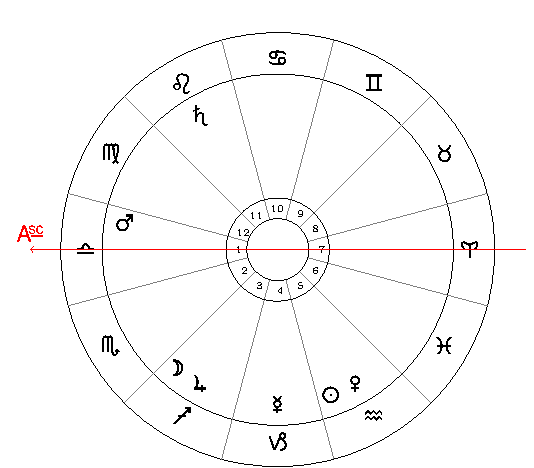
\includegraphics[width=.68\textwidth]{charts/5_10_10}
\caption{Chart 65 [V.10.10, GH L122,I,22]}
\label{fig:chart65}
\end{wrapfigure}

\noindent Another example: \Sun, \Venus\xspace in \Aquarius, \Moon, \Jupiter\xspace in \Sagittarius, \Saturn\xspace in \Leo, \Mercury\xspace in \Capricorn, \Mars, Ascendant in \Libra\footnote{\textit{Gree Horoscopes} dates the chart to January 22, 122 CE at about 10 p.m.}. 

In his 35th year he was in danger of prison because of riot and
violence: the \Moon\xspace was sextile with \Mars, and \Mars\xspace itself had received the year from the \Moon\xspace and had transmitted it to \Saturn. These successive transmissions are grievous and dangerous. But \Jupiter\xspace was with the \Moon\xspace and received the year from the \Sun\xspace and \Venus, who were in the <V> Place associated with friends. \Jupiter\xspace happened to be in the Place of Travel and caused travel which was voluntary but risky, as well as help from and associations with friends.

\begin{wrapfigure}[15]{R}{7cm}
\centering
\vspace{-20pt}
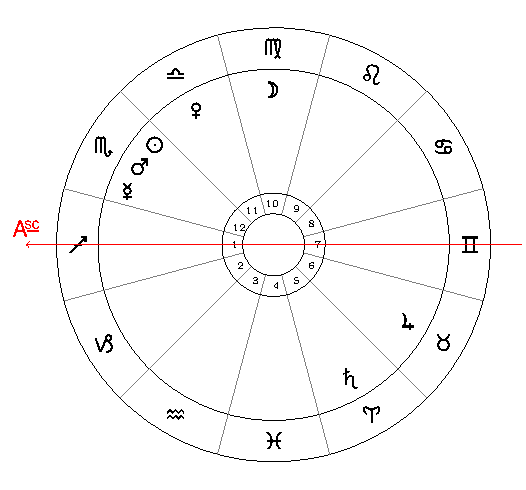
\includegraphics[width=.68\textwidth]{charts/5_10_11}
\caption{Chart 66 [V.10.11, GH L114,XI]}
\label{fig:chart66}
\end{wrapfigure}

\noindent Another example: \Sun, \Mars, \Mercury\xspace in \Scorpio, \Saturn\xspace in \Aries, \Moon\xspace in \Virgo, \Jupiter\xspace in \Taurus, \Venus\xspace in \Libra, Ascendant in \Sagittarius\footnote{\textit{Greek Horoscopes} dates the chart to November 10, 114 CE at about 8 a.m.}. 

In his 42nd year he experienced troubles, confusion, and scandal
because of a woman. 

\noindent In his 44th year the violent death of a slave, a crisis for his father, and an accusation of base descent and of violence. But he got help and gifts from friends. He had troubles related \textbf{/231K/} to documents; he experienced penalties, assaults, and false accusations. He suffered grief because of his slaves and he had problems with his health. We see that each transmission had its own influence, and likewise each Place.

\begin{wrapfigure}[14]{R}{7cm}
\centering
\vspace{0pt}
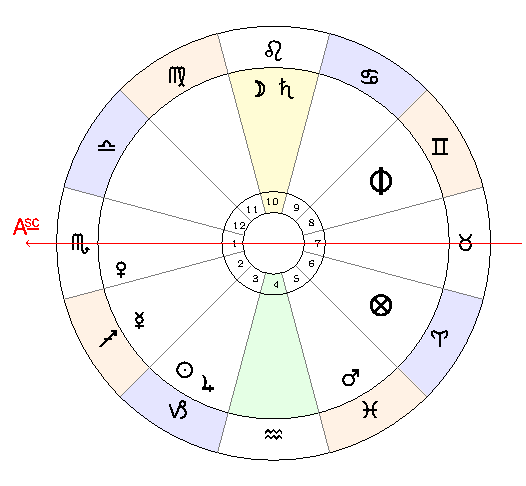
\includegraphics[width=.68\textwidth]{charts/5_10_12}
\caption{Chart 67 [V.10.12, GH L123,I]}
\label{fig:chart67}
\end{wrapfigure}

Another example: \Sun, \Jupiter\xspace in \Capricorn, \Moon, \Saturn\xspace in \Leo, \Mars\xspace in \Pisces, \Venus, Ascendant in \Scorpio, \Mercury\xspace in \Sagittarius\footnote{\textit{Greek Horoscopes} dates the chart to January 3, 123 CE at about 2 a.m.}. 

The Crisis-producing Places were found in \Pisces\xspace and \Scorpio, because \Venus\xspace was in \Scorpio\xspace and \Mars in Pisces. He was a dancer, and in his 20th year he was taken into custody during a mob uprising. He, however, was defended before the governor by the help of his friends. He was released through the pleas of the crowd and became even more famous. The transmission of the year was from \Saturn\xspace and the \Moon\xspace to \Mars\xspace and the Crisis-producing Place <by 8 signs>, and from \Jupiter\xspace and the \Sun\xspace in the III Place concerned with property to \Saturn\xspace and the \Moon\xspace at MC, in the X Place, a Place associated with occupations. 

In addition the distribution by 4 signs, i.e. from \Saturn\xspace and the \Moon\xspace to \Venus\xspace and the Ascendant, is indicative of the riot, the quarrelsomeness, and the rivalry throughout the affair, as is the distribution by 4 signs, from \Mercury\xspace to \Mars\xspace and the Crisis-producing Place (4 signs). All the stars were operative in his 20th year, and so the nativity was in danger of loss of rank, of \textbf{/220P/} condemnation, and of loss of life. Since, however, \Venus\xspace was found in the Ascendant and <\Mars> in the Crisis-producing Place, while \Jupiter\xspace was with the \Sun, the native had a spectacular escape and gained
success from this affair. In addition the Lot of Fortune was in \Aries\xspace and the ruler of the exaltation of the nativity, the \Sun <in \Capricorn>, was at MC relative to the Lot of Fortune, as was \Mars\xspace relative to Daimon <in \Gemini>. 

Later in his 32nd year he lost his office, his rank, and his livelihood, and lived in disgrace, since the Lot of Fortune happened to be preceding an angle, and \Saturn\xspace was at MC, not in its own sect, and in opposition to the <11th> Place of Accomplishment in \Aquarius, \Saturn’s own house. As a result he caused his own downfall, being arrogant and boastful. \Mercury, the ruler of Daimon, the Intellectual Place, was in opposition to itself in \Gemini <a house of \Mercury>.

\begin{wrapfigure}[15]{R}{7cm}
\centering
\vspace{-20pt}
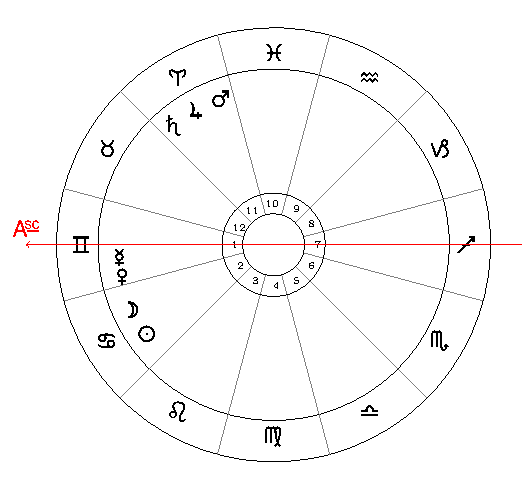
\includegraphics[width=.68\textwidth]{charts/5_10_13}
\caption{Chart 68 [V.10.13, GH L113,VII]}
\label{fig:chart68}
\end{wrapfigure}

\noindent Another example: \Sun, \Moon, in \Cancer, \Saturn, \Jupiter, \Mars\xspace in \Aries, \Venus, \Mercury, Ascendant in \Gemini\footnote{{Greek Horoscopes} dates the chart to July 1, 113 CE at about 4 a.m.}. 

In his 20th year both his parents were killed while attending a festival by an attack of bandits, because the transmission was from the Ascendant to the <VIII> Place of Death <\Capricorn>. Even more operative was the transmission by 4 signs from \Saturn\xspace and \Mars\xspace to the \Sun\xspace and \Moon, which were in the
<II> Place associated with death \textbf{/232K/} and which indicated the father and mother. The native, however, escaped danger in the uproar, so as to show that the transmission from \Jupiter\xspace <to the \Sun\xspace and \Moon> was also powerful at the same time.
\newpage